\documentclass[utf8x]{beamer}

\mode<presentation>
{
  \usetheme{Warsaw}

  %\setbeamercovered{transparent}
}


\usepackage[english]{babel}

\usepackage[utf8x]{inputenc}

\usepackage{times}
\usepackage[T1]{fontenc}

\title[Back to the Future in one Week]
{%
    Back to the Future in one Week — Implementing a Smalltalk VM in PyPy%
}

\author[Bolz, Kuhn, Lienhard, Matsakis, Nierstrasz, Renggli, Rigo, Verwaest]
{
    \textcolor{green!50!black}{Carl~Friedrich~Bolz}\inst{1} \and
    Adrian~Kuhn\inst{2} \and
    Adrian~Lienhard\inst{2} \and
    Nicholas~D.~Matsakis\inst{3} \and
    Oscar~Nierstrasz\inst{2} \and
    Lukas~Renggli\inst{2} \and
    Armin~Rigo \and
    Toon~Verwaest\inst{2}
}

\institute[Bern and others]
{
    \inst{2}%
    Software Composition Group\\ University of Bern, Switzerland
    \and%
    \vskip-2mm
    \inst{1}
    Softwaretechnik und Programmiersprachen\\ Heinrich-Heine-Universit\"at D\"usseldorf
    \and%
    \vskip-2mm
    \inst{3}%
    ETH Zurich, Switzerland
}


\date{Workshop on Self-sustaining Systems, May 16 2008}


% Delete this, if you do not want the table of contents to pop up at
% the beginning of each subsection:
%\AtBeginSubsection[]
%{
%  \begin{frame}<beamer>
%    \frametitle{Outline}
%    \tableofcontents[currentsection,currentsubsection]
%  \end{frame}
%}


% If you wish to uncover everything in a step-wise fashion, uncomment
% the following command: 

%\beamerdefaultoverlayspecification{<+->}


\begin{document}

\begin{frame}
  \titlepage
\end{frame}

%\begin{frame}
%  \frametitle{Outline}
%  \tableofcontents
  % You might wish to add the option [pausesections]
%\end{frame}

\begin{frame}
    \frametitle{Scope}
    This talk is about: XXX
    \begin{itemize}
    \item writing a Squeak implementation
    \item with eight people
    \item in five days
    \item using PyPy
    \end{itemize}
\end{frame}

\begin{frame}
    \frametitle{What is PyPy}
    \begin{itemize}
    \item started as a Python implementation in Python
    \item developed into a general environment for implementing dynamic languages
    \item supports the language developer with a lot of infrastructure
    \item Open Source project, MIT license
    \item most important goal: abstracting over low-level details
    \item don't fix decisions about low-level details 
    \end{itemize}
\end{frame}

\begin{frame}
    \frametitle{PyPy's Approach to VM Construction}
    \begin{itemize}
    \item implement an interpreter for the dynamic language in RPython
    \item translate this interpreter to a low-level language
    \item translating inserts low-level details
    \item a variety of target environment: C, LLVM, JVM, .NET
    % XXX write about model-driven development?
    \end{itemize}
    \pause
    \begin{block} {What is RPython?}
        \begin{itemize}
        \item a more static subset of Python
        \item static enough to enable type inference
        \item still rather expressive: exceptions, inheritance, dynamic dispatch
        \item analysis starts after importing of interpreter
        \item enables compile-time metaprogramming
        \end{itemize}
    \end{block}
\end{frame}

\begin{frame}
    \begin{block} {Translation Aspects}
        \begin{itemize}
        \item many aspects of the final VM are orthogonal to language semantics
        \item examples: GC strategy, threading model, many object details
        \item non-trivial translation aspect: auto-generating a dynamic compiler
        \item those shouldn't manifest in the interpreter source
        \item they are inserted during translation
        \end{itemize}
    \end{block}
    \pause
    \begin{block} {Compile-Time Metaprogramming}
        \begin{itemize}
        \item PyPy's translation toolchain starts analysis after importing
        \item arbitrary (non-RPython) code can be executed during import
        \item this allows metaprogramming of parts of the interpreter
        \end{itemize}
    \end{block}
\end{frame}

\begin{frame}
    \frametitle{The SPy VM}
    \begin{itemize}
        \item really simple, straight-forward Squeak interpreter in RPython
        \item essentially free of low-level details, no GC
        \item written in the course of five days
        \item sprint-driven development
    \end{itemize}
    \pause
    \begin{block} {Status}
        \begin{itemize}
        \item bytecodes fully implemented
        \item many primitives implemented: arithmetic primitives, object primitives
        \item can load Squeak images by decoding the bit patterns
        \item runs simple benchmarks
        \end{itemize}
    \end{block}
\end{frame}

\begin{frame}
    \frametitle{SPy Object Model}
    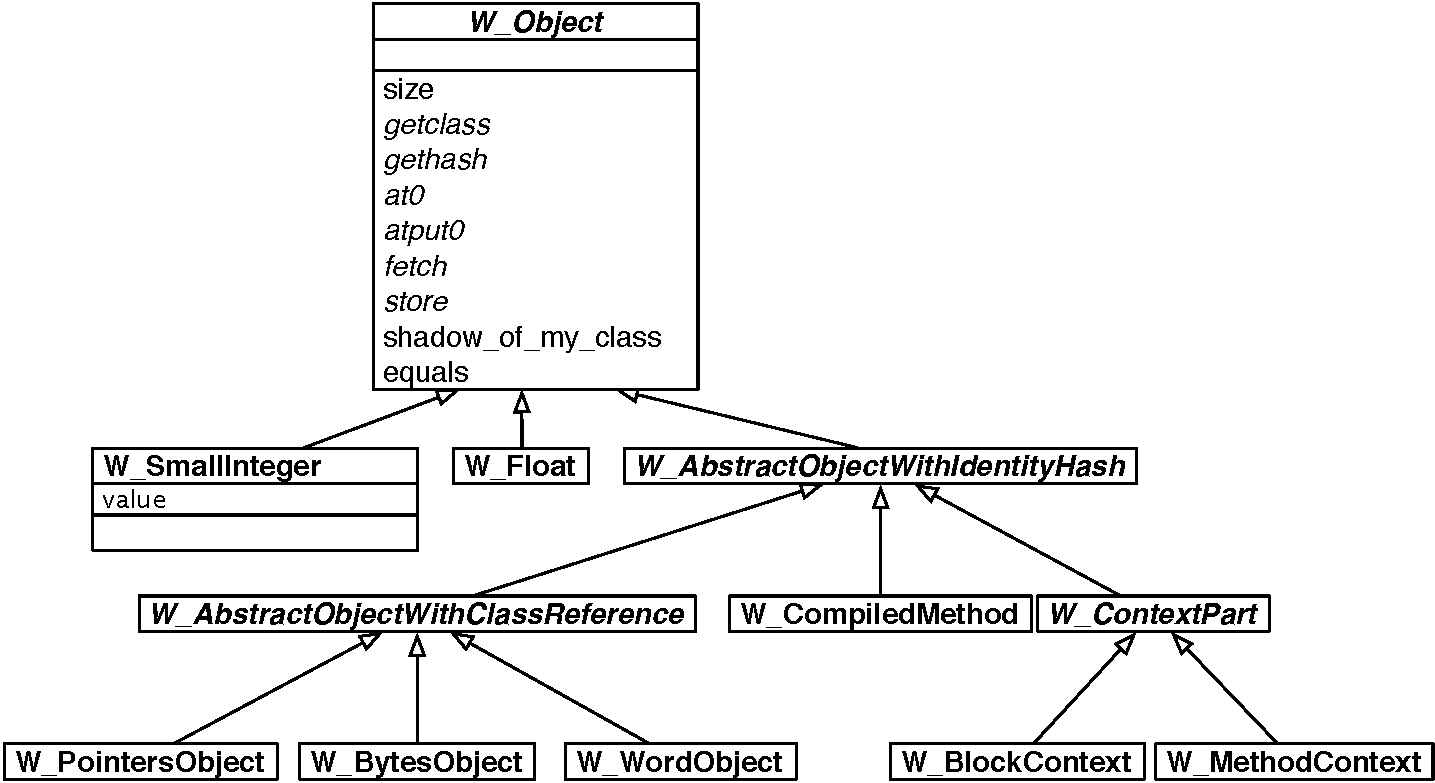
\includegraphics[height=5cm]{objmodel}
\end{frame}

\begin{frame}
    \frametitle{Shadows}
    Problem: 
    \begin{itemize}
    \item classes are just objects: can't really say which objects are used as classes
    \item any object with the right instance fields can be used as a class
    \item cryptic bitfields in the class which the VM needs to decode all the time
    \end{itemize}
    \pause
    \begin{block}{Shadows}
        \begin{itemize}
        \item approach: potentially attach a \emph{shadow} to every object
        \item the shadow caches VM-internal information
        \item when the object is changed, the shadow is invalidated
        \item so far only used for classes, later contexts, methods
        \item conceptual cleanliness and nicer VM implementation
        \end{itemize}
    \end{block}
\end{frame}

\begin{frame}
    \frametitle{Tagged Pointers}
    \begin{itemize}
    \item Squeak implements integers as tagged pointers
    \item doing that is orthogonal to language semantics
    \item in PyPy implemented as a translation aspect
    \item one class with exactly one int field can be implemented with a flag
    \item when enabled, all method calls check for tag first
    \item usually changing such a decision would be a major effort
    \end{itemize}
    \pause
    \begin{block}{Results}
        \begin{itemize}
        \item small slowdown
        \item memory advantage not measured
        \item really easy to do
        \end{itemize}
    \end{block}
\end{frame}

\begin{frame}
    \frametitle{Primitives}
    \begin{itemize}
    \item try to make writing primitives easy
    \item failure signaled by an exception
    \item automatic popping from the stack and unwrapping of arguments
    \item automatic pushing of the result
    \item using a custom decorator \texttt{expose\_primitive}
    \item compile-time metaprogramming
    \end{itemize}
\end{frame}

\frame[containsverbatim, plain, shrink=10]{
  \begin{verbatim}
bool_ops = [
    (LESSTHAN, operator.lt),
    (GREATERTHAN, operator.gt),
    (LESSOREQUAL, operator.le),
    (GREATEROREQUAL,operator.ge),
    (EQUAL, operator.eq),
    (NOTEQUAL, operator.ne)
    ]


def make_func(code, op):

    @expose_primitive(code, unwrap_spec=[int, int])
    def func(interp, v1, v2):
        res = op(v1, v2)
        w_res = utility.wrap_bool(res)
        return w_res

for (code, op) in bool_ops:
    make_func(code, op)
  \end{verbatim}
}

\begin{frame}
    \frametitle{Image Loading}
    \begin{itemize}
    \item manual decoding of Squeak images by reading Squeak object format
    \item image writing could be done in the same way later
    \item not really a reason to directly use a memory dump
    \item (hard anyway, on object-oriented platforms)
    \end{itemize}
\end{frame}

\frame[plain]{
    \frametitle{Performance (tiny Benchmark)}
    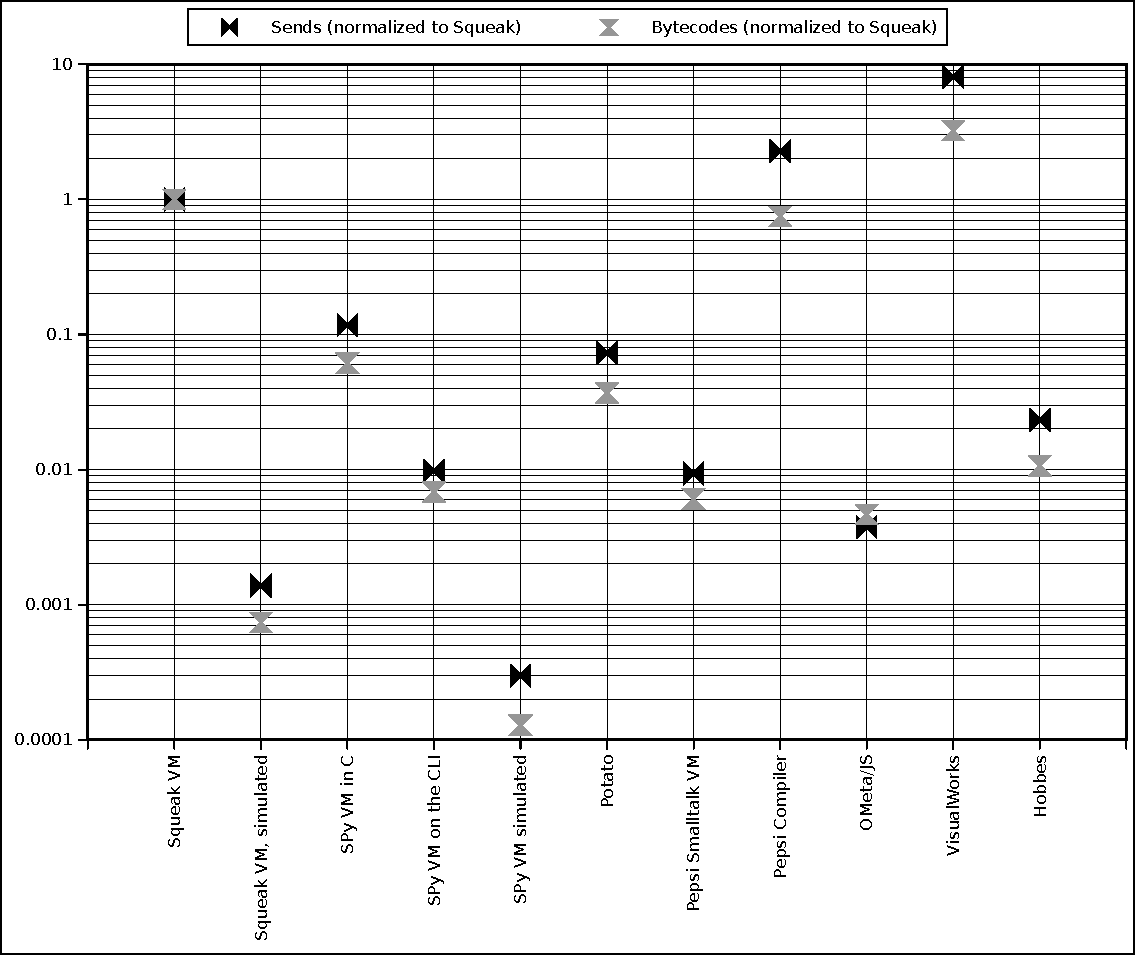
\includegraphics[height=8cm]{speed}
}

\begin{frame}
    \frametitle{Results}
    {\bf Good Points of the Approach:}
    \begin{itemize}
    \item simple, understandable, high-level Squeak implementation
    \item mostly free of low-level details: no GC, no manual pointer tagging
    \item written in a short amount of time
    \item runs on various platforms
    \end{itemize}
    \pause
    {\bf Bad Points of the Approach:}
    \begin{itemize}
    \item not really fast (yet)
    \item XXX XXX
    \end{itemize}
\end{frame}

\begin{frame}
    \frametitle{Outlook}
    \begin{itemize}
    \item do graphical builtins, to actually start the full environment
    \item Squeak-specific optimizations:
    \item method-cache (should be easy with shadows)
    \item JIT (see next slide)
    \item lessons learned for a "SqueaSquea"?
    \end{itemize}
\end{frame}

\begin{frame}
    \frametitle{JIT Outlook}
    \begin{itemize}
    \item PyPy currently explores automatic JIT generation
    \item almost orthogonal from the interpreter source – applicable to many
          languages, follows language evolution ``for free''
    \item based on Partial Evaluation techniques
    \item benefits from a high-level interpreter
    \item generating a dynamic compiler is easier than generating a static one!
    \item shares ideas with tracing JITs
    \pause
    \item current status: basic ideas seem to work, good speedups in prototypes
    \item a lot of details still left
    \end{itemize}
\end{frame}

\begin{frame}
  \frametitle{Questions?}
  \begin{block}{
    PyPy}
    \bigskip
    \hskip 1cm \url{http://codespeak.net/pypy/}
    \bigskip
  \end{block}
\end{frame}

\end{document}
